%!TEX root = ../main.tex

\chapter{Literature Review\label{chap:literature_review}}

\section{Traditional word embedding methods}

\subsection{Word2Vec}
Word2Vec \cite{mikolov2013efficient} is algorithm that generates word embedding using information about target word (context).
Word2Vec uses \ac{NN} and \ac{ML} techniques to generate word embedding for every word in vocabulary during training.
As \ac{NN} architecture are used \ac{CBOW} and Skip-gram, \reffig{fig:cbow_skipgram_scheme}.

\begin{figure}[h]
    \centering
    \begin{tikzpicture}[
    framed,
    squarednode/.style={rectangle, draw=black!60, very thick, minimum size=5mm},
    emptysquare/.style={squarednode, draw=none},
    largedrectangle/.style={squarednode, minimum width=10mm, minimum height=15mm},
    emptyrectangle/.style={squarednode, draw=none,minimum width=10mm},
    ]
    %Nodes
    \node[emptysquare]     (input3)  []                 {};
    \node[squarednode]     (input2)  [above=of input3]  {};
    \node[squarednode]     (input1)  [above=of input2]  {};
    \node[squarednode]     (input4)  [below=of input3]  {};
    \node[squarednode]     (input5)  [below=of input4]  {};
    \node[largedrectangle] (sum)     [right=of input3]  {SUM};
    \node[emptyrectangle]  (sum3)    [right=of input3]  {};
    \node[emptyrectangle]  (sum2)    [above=of sum3]    {};
    \node[emptyrectangle]  (sum1)    [above=of sum2]    {};
    \node[squarednode]     (output)  [right=of sum]     {};
    \node[emptysquare]     (output2) [above=of output]  {};
    \node[emptysquare]     (output1) [above=of output2] {};
    
    % Text labels (outside nodes)
    \node[left=of input1.east, xshift=3mm] {w(t-2)};
    \node[left=of input2.east, xshift=3mm] {w(t-1)};
    \node[left=of input4.east, xshift=3mm] {w(t+1)};
    \node[left=of input5.east, xshift=3mm] {w(t+2)};
    \node[below=of output.north]           {w(t)};
    \node[above=of input1.north]           {Input};
    \node[above=of sum1.north]             {Projection};
    \node[above=of output1.north]          {Output};

    %Lines
    \draw[->] (input1.east) -- (sum.west);
    \draw[->] (input2.east) -- (sum.west);
    \draw[->] (input4.east) -- (sum.west);
    \draw[->] (input5.east) -- (sum.west);
    \draw[->] (sum.east)    -- (output.west);
\end{tikzpicture}
    \begin{tikzpicture}[
    framed,
    squarednode/.style={rectangle, draw=black!60, very thick, minimum size=5mm},
    emptysquare/.style={squarednode, draw=none},
    largedrectangle/.style={squarednode, minimum width=10mm, minimum height=15mm},
    emptyrectangle/.style={squarednode, draw=none,minimum width=10mm},
    ]
    %Nodes
    \node[squarednode]     (input3)  []                 {};
    \node[emptysquare]     (input2)  [above=of input3]  {};
    \node[emptysquare]     (input1)  [above=of input2]  {};
    \node[emptysquare]     (input4)  [below=of input3]  {};
    \node[emptysquare]     (input5)  [below=of input4]  {};
    \node[largedrectangle] (sum)     [right=of input3]  {};
    \node[emptyrectangle]  (sum3)    [right=of input3]  {};
    \node[emptyrectangle]  (sum2)    [above=of sum3]    {};
    \node[emptyrectangle]  (sum1)    [above=of sum2]    {};
    \node[emptysquare]     (output3) [right=of sum]     {};
    \node[squarednode]     (output2) [above=of output3] {};
    \node[squarednode]     (output1) [above=of output2] {};
    \node[squarednode]     (output4) [below=of output3] {};
    \node[squarednode]     (output5) [below=of output4] {};
    \node[emptysquare]     (output1) [above=of output2] {};
    
    % Text labels (outside nodes)
    \node[below=of input3.north]  {w(t)};
    \node[right=of output1.west]  {w(t-2)};
    \node[right=of output2.west]  {w(t-1)};
    \node[right=of output4.west]  {w(t+1)};
    \node[right=of output5.west]  {w(t+2)};
    \node[above=of input1.north]  {Input};
    \node[above=of sum1.north]    {Projection};
    \node[above=of output1.north] {Output};

    %Lines
    \draw[->] (input3.east) -- (sum.west);
    \draw[->] (sum.east)    -- (output1.west);
    \draw[->] (sum.east)    -- (output2.west);
    \draw[->] (sum.east)    -- (output4.west);
    \draw[->] (sum.east)    -- (output5.west);
\end{tikzpicture}
    \caption{\ac{CBOW} and Skip-gram schemes respectively}
    \label{fig:cbow_skipgram_scheme}
\end{figure} 

Due to its algorithmic simplicity and efficiency, Word2Vec has established itself as a strong baseline for numerous \ac{NLP} tasks.
Compared to more recent and complex models, Word2Vec requires minimal hyperparameter tuning, making it a relatively straightforward approach.

However, it is important to acknowledge that Word2Vec has limitations.
These include its inability to capture \textbf{global information} within a document, its challenges in effectively handling \textbf{morphologically rich languages} (languages with many word variations), and its lack of awareness of the \textbf{broader context} beyond a limited window of surrounding words.

\subsection{\acf{GloVe}}
\ac{GloVe} \cite{pennington2014glove} leverages the co-occurrence statistics of words within a corpus to learn vector representations.
This approach involves constructing a co-occurrence matrix, where each entry reflects the frequency of two words appearing together within a predefined window size.
This matrix essentially captures the relative importance of various word pairings.

A core principle of \ac{GloVe} lies in the notion that word vectors should effectively encode the ratios between co-occurrence probabilities of words.
By analyzing these ratios, \ac{GloVe} can identify semantic relationships between words.
This is achieved by factorizing the co-occurrence matrix into a lower-dimensional space, allowing for efficient representation and manipulation of word meanings.

To optimize the learned word embeddings, \ac{GloVe} employs a weighted least squares objective function.
This function aims to minimize the discrepancy between the dot product of two word vectors and the logarithm of their co-occurrence probability.
Through iterative adjustments of the word vectors, \ac{GloVe} converges on a solution that yields the desired word embeddings.

\subsection{FastText}
FastText \cite{bojanowski2017enriching} utilizes similar \ac{NN} architectures as Word2Vec, namely \ac{CBOW} and Skip-gram, but applies them to character n-grams (subwords) instead of entire words.
This decomposition allows FastText to represent a word's meaning by considering its constituent subword components.
Consequently, FastText offers advantages in two key areas:
\begin{itemize}
    \item \textbf{Rare Word Embeddings}: Unlike Word2Vec, which struggles with words appearing infrequently in the training data, FastText can construct meaningful representations for rare words. By leveraging known subwords, FastText can represent unseen words, making it particularly valuable for working with large and diverse datasets.    
    \item \textbf{Handling Morphologically Rich Languages}: Languages with complex morphology, where words are formed through prefixes and suffixes, often pose challenges for Word2Vec. FastText overcomes this limitation by capturing the shared subwords between derived words and their root forms. This allows FastText to represent the inherent relationships between words in these languages, leading to more accurate \ac{NLP} tasks.
\end{itemize}
However, it's important to acknowledge that FastText also has limitations:
\begin{itemize}
    \item \textbf{Context Insensitivity}: Similar to Word2Vec, FastText embeddings do not inherently capture the order or context in which words appear within a sentence. This can be a drawback for tasks like sentiment analysis or machine translation, where word order and context are crucial for accurate interpretation.
    \item \textbf{Limited Long-Range Dependency Capture}: While subwords allow FastText to capture local context, it might not effectively capture long-range dependencies within sentences. This can be a disadvantage for tasks requiring analysis of complex sentence structures, where understanding the relationships between words across larger distances is important.    
\end{itemize}

\section{Transformer-based models}
Transformer models \cite{vaswani2023attention} \nocite{umarjamilai} underpin powerful \ac{NLP} models like \ac{BERT}.
A key advantage is their self-attention mechanism, which assigns importance to words based on context, not just position.
This enables efficient parallel processing of entire sentences.
Architecture of transformers visualized in \reffig{fig:model-arch}

\begin{figure}[h]
    \centering
    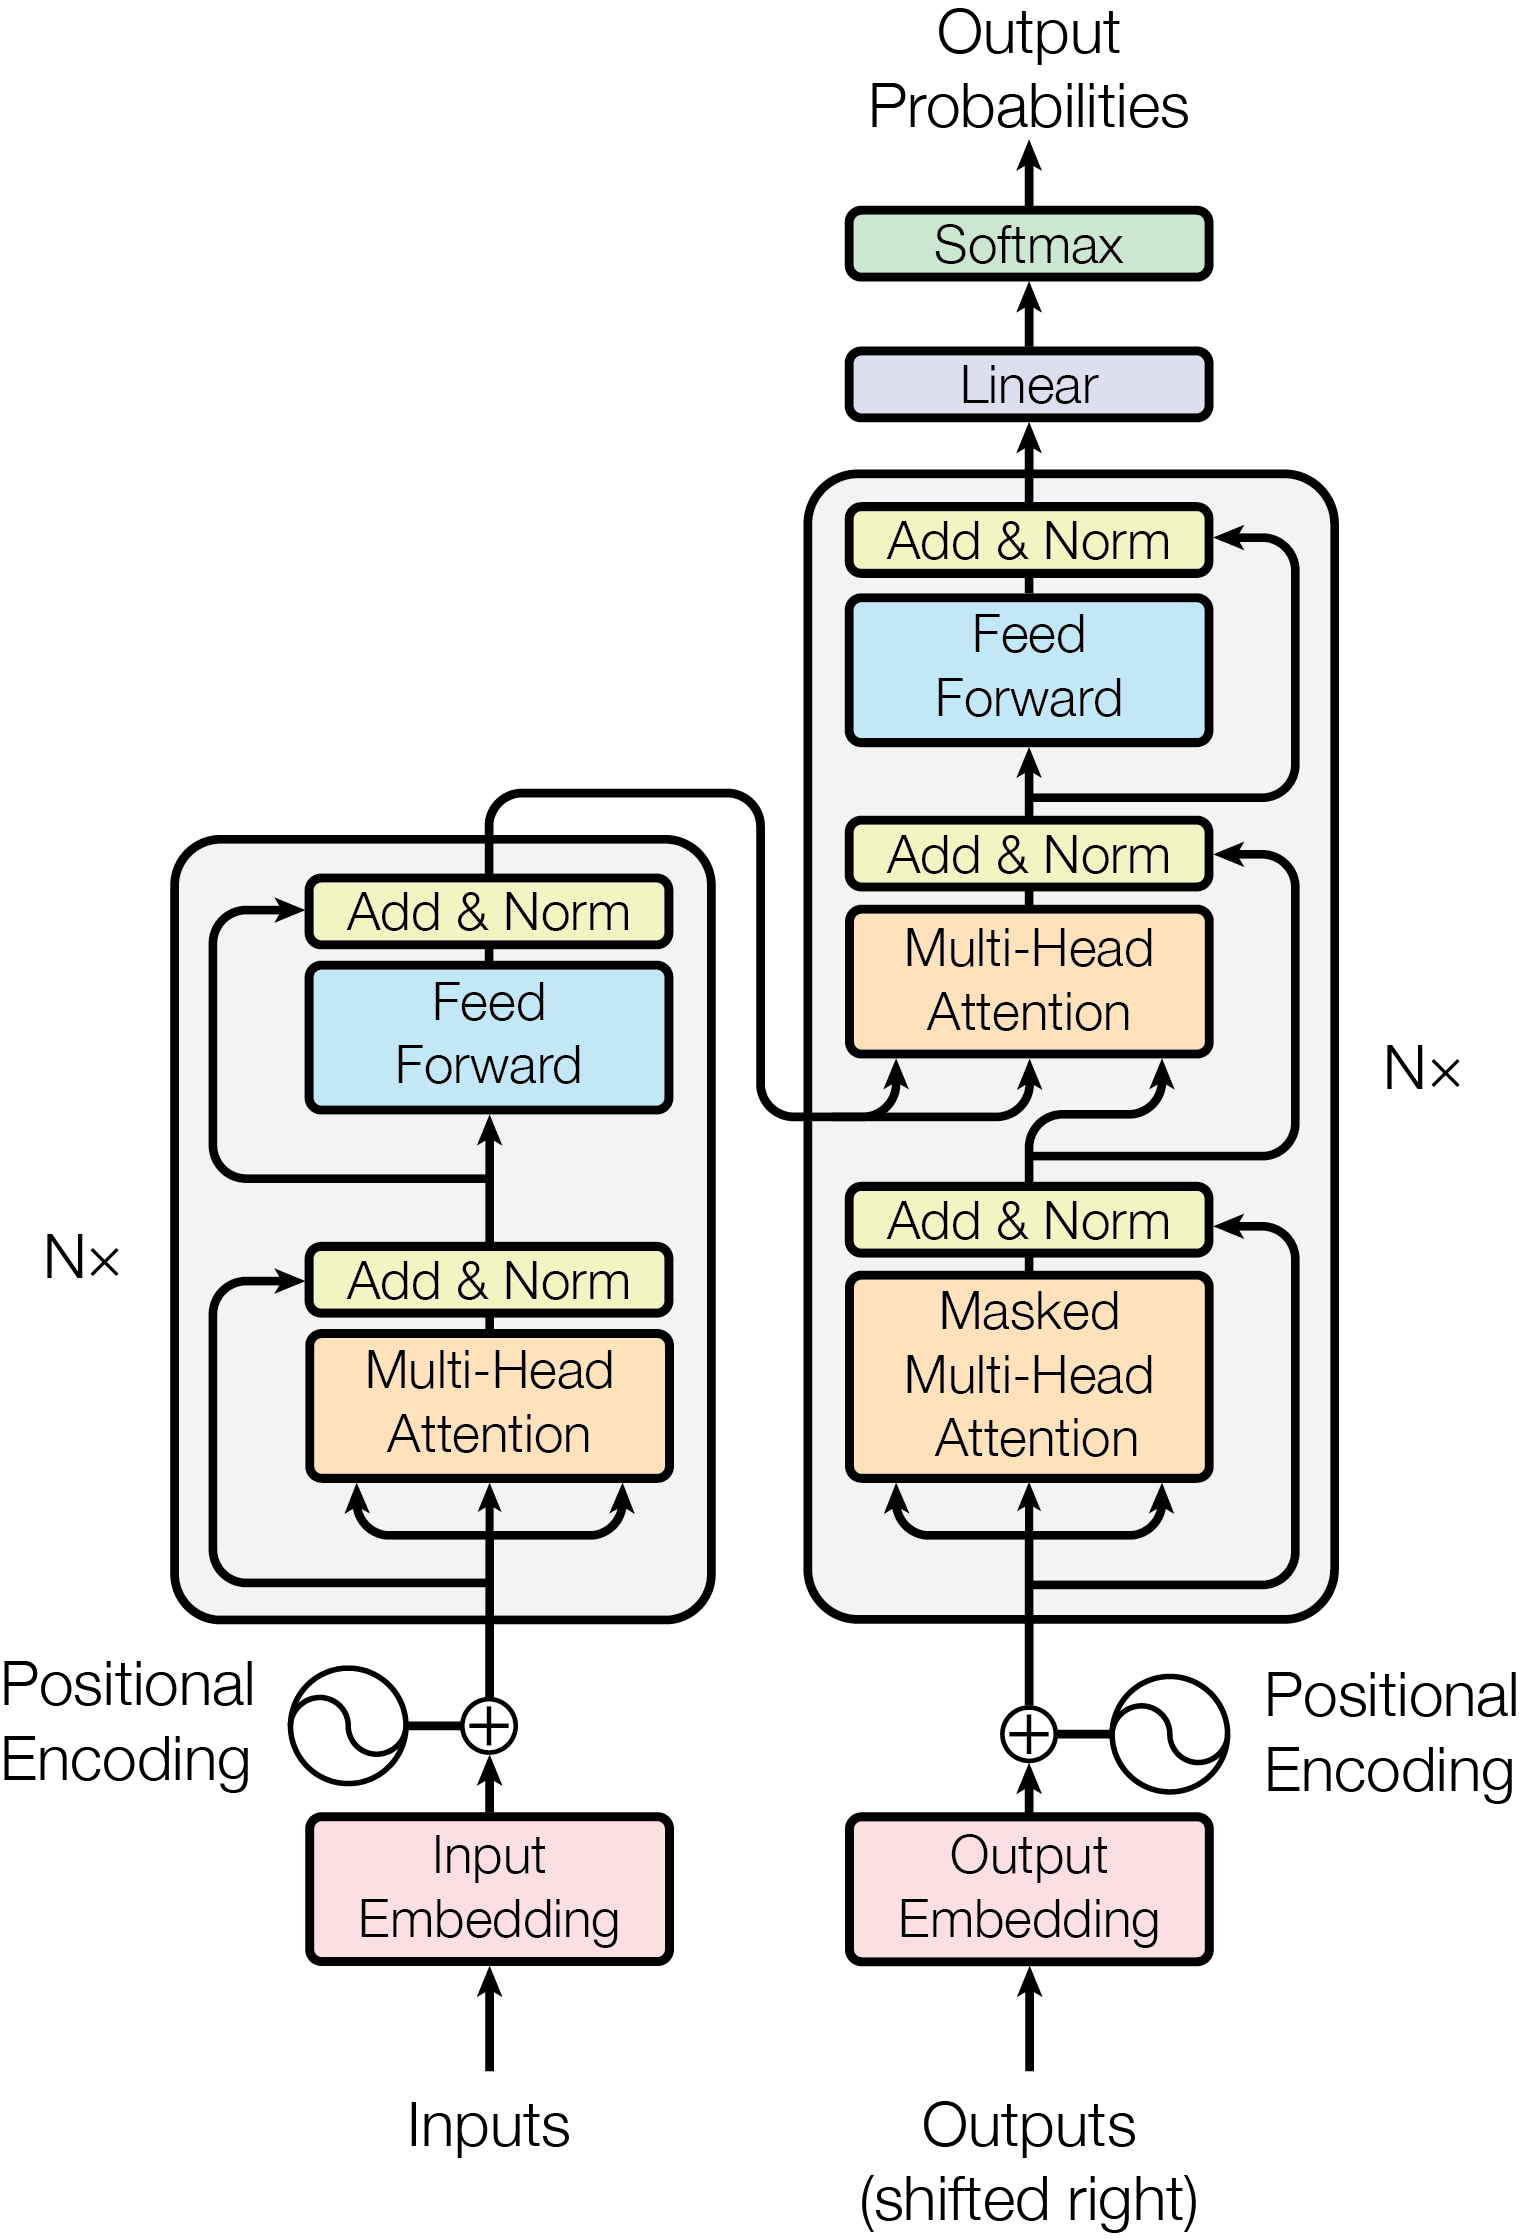
\includegraphics[scale=0.6]{src/fig/imgs/transformer_arch.png}
    \caption{The Transformer - model architecture.}
    \label{fig:model-arch}
\end{figure}

\ac{BERT} \cite{devlin2019bert} builds on transformers with pre-training on a massive text corpus.
\ac{MLM} and \ac{NSP} further enhance \ac{BERT}'s capabilities, fostering deep contextual understanding and grasp of sentence relationships.
\ac{MLM} injects a deeper understanding of context into \ac{BERT} by requiring it to predict masked words within a sentence.
Through this process, \ac{BERT} learns the relationships between words and their meaning based on the surrounding context.
This goes beyond simple memorization - it allows \ac{BERT} to grasp the nuances of language and handle even unseen words.
\ac{NSP}, on the other hand, strengthens \ac{BERT}'s ability to understand the flow and connection between sentences.
During training, \ac{BERT} is presented with sentence pairs and tasked with determining if the second sentence logically follows the first. 
By tackling this objective, \ac{BERT} develops a grasp of sentence relationships, enabling it to analyze and process text that unfolds across multiple sentences, like news articles or conversations.

These strengths make transformers, particularly \ac{BERT}, well-suited for \ac{NLP} tasks.
Their advantage lies in capturing contextual understanding, leading to richer text representations and superior comprehension of semantic relationships.

Furthermore, \ac{BERT} excels in transfer learning, readily adapting to various tasks (sentiment analysis, \ac{QA}) with minimal modifications.
Additionally, efficiency and speed are benefits due to parallel processing and pre-training.

Transformer models effectiveness is validated by state-of-the-art performance across \ac{NLP} benchmarks.
Finally, \ac{BERT}'s robustness allows it to handle nuances in text without significant performance degradation.

\section{Methods of text representations evaluation}

\subsection{Analogy tests}

Analogy tests, as demonstrated in the seminal Word2Vec paper \cite{mikolov2013efficient}, are a widely used method for assessing the quality of text representations, particularly word embeddings.
These tests evaluate whether the semantic relationships between words are effectively captured and preserved within the vector space employed by the model.

A typical analogy test question follows the format "A is to B as C is to D," where A, B, C, and D represent words.
For instance, the question "man is to king as woman is to queen" probes the model's understanding of gender relations.
If the word embeddings are of high quality, performing the vector operation vector(king) - vector(man) + vector(woman) should result in a vector that closely resembles vector(queen).
This outcome indicates that the model has successfully learned the analogous relationship between "man" and "king" and "woman" and "queen."

\subsection{Confusion matrix}

Confusion matrices are a widely used tool for evaluating classification algorithms, and they can be adapted to assess text representations in tasks such as word sense disambiguation, part-of-speech tagging, or sentiment analysis.
A confusion matrix is a table that describes the performance of a classification model by comparing predicted and actual labels.

\section{\acf{RAG}}
\ac{RAG} \cite{lewis2021retrievalaugmented} \nocite{umarjamilai} is an advanced \ac{NLP} framework that combines the strengths of retrieval-based and generation-based models to produce high-quality, contextually relevant text based on provided document (web-page etc.), instruction and query (question). 

\subsection{Architecture of \ac{RAG}}
The \ac{RAG} algorithm leverages a two-stage approach for answer generation: retrieval and generation.
Both stages rely heavily on the chosen text representation technique.

\begin{itemize}
  \item \textbf{Retrieval}:
    In the initial phase, the algorithm extracts relevant information from the document and splits it into manageable chunks.
    These chunks are then fed into text representation models, which convert them into a format suitable for efficient retrieval.
    This process results in encoded representations of the information, which are then stored within a vector database.
    During the retrieval phase, \ac{RAG} utilizes the same text representation model to encode the user's query (question).
    Subsequently, it searches the vector database and identifies the top-$K$ most relevant passages based on their encoded representations.
  \item \textbf{Generation}:
    The $K$ retrieved passages identified in the information retrieval phase serve as crucial contextual information for the \ac{LLM} within the \ac{RAG} system.
    By providing this context alongside the user's question and any additional instructions, the \ac{LLM} is empowered to generate a comprehensive and informative answer.
\end{itemize}

Architecture of the \ac{RAG} algorithm is shown on the \reffig{fig:RAG_scheme}

\begin{figure}[h]
  \centering
  % Inspired by:
% https://en.m.wikipedia.org/wiki/File:RAG_schema.svg
% https://github.com/hkproj/retrieval-augmented-generation-notes/blob/main/Slides.pdf

\begin{tikzpicture}[
    longnode/.style={rectangle, rounded corners=.5em, draw=black!60, very thick, align=left, minimum height=1.7em, minimum width=9em},
    emptylong/.style={longnode, draw=none},
    highnode/.style={longnode, minimum height=10.2em},
    line width=1pt, black
    ]
    
    %Nodes
    \node[longnode]  (question)    []                     {Question};
    \node[emptylong] (empty1)      [below=of question]    {};
    \node[longnode]  (embeddings1) [below=of empty1]      {Embeddings};
    \node[longnode]  (vector_db)   [right=of embeddings1] {Vector database};
    \node[longnode]  (embeddings2) [below=of vector_db]   {Embeddings};
    \node[longnode]  (chunks)      [below=of embeddings2] {Split into chunks};
    \node[longnode]  (documents)   [below=of chunks]      {Documents};
    \node[longnode]  (context)     [right=of vector_db]   {Context};
    \node[longnode]  (instruction) [above=of context]     {Instruction};
    \node[emptylong] (llm_empty3)  [right=of context]     {};
    \node[emptylong] (llm_empty2)  [above=of llm_empty3]  {};
    \node[emptylong] (llm_empty1)  [above=of llm_empty2]  {};
    \node[highnode]  (LLM)         [right=of instruction] {LLM};
    \node[longnode]  (answer)      [below=of llm_empty3]  {Answer};

    %Lines
    \draw[->] (question.south)    --                                                  (embeddings1.north);
    \draw[->] (embeddings1.east)  -- node[text width=3em,midway,above=0.7em] {Search} (vector_db.west);
    \draw[->] (embeddings2.north) -- node[text width=3em,midway,right=0.7em] {Store}  (vector_db.south);
    \draw[->] (chunks.north)      --                                                  (embeddings2.south);
    \draw[->] (documents.north)   --                                                  (chunks.south);
    \draw[->] (vector_db.east)    -- node[text width=3em,midway,above=0.7em] {Top-K}  (context.west);
    \draw[->] (context.east)      --                                                  (llm_empty3.west);
    \draw[->] (instruction.east)  --                                                  (llm_empty2.west);
    \draw[->] (question.east)     --                                                  (llm_empty1.west);
    \draw[->] (llm_empty3.south)  --                                                  (answer.north);
\end{tikzpicture}
  \caption{Retrieval-Augmented Generation architecture.}
  \label{fig:RAG_scheme}
\end{figure}

\subsection{Factors influencing \ac{RAG} performance}
The performance of \ac{RAG} systems can be influenced by several key factors.
Two important aspects are:

\begin{itemize}
    \item \textbf{Embedding Model Selection}:
        Previous work \cite{joshi2024RAGemb} suggests that the choice of embedding model significantly impacts \ac{RAG} performance.
        Different embedding models offer varying strengths in capturing semantic relationships within text data.
        Selecting the most suitable model depends on the specific task and dataset.
    \item \textbf{Document Chunking Size}:
        Another factor influencing \ac{RAG} performance is the size of the document chunks used for retrieval \cite{theja2023RAGchunk}.
        Splitting documents into smaller chunks can potentially improve retrieval efficiency.
        However, excessively small chunks may lead to a loss of context and hinder the \ac{RAG} system's ability to generate coherent and relevant text.
        Finding the optimal chunking size requires careful consideration of the task and available computational resources.    
\end{itemize}




% Literature Review Structure
% \begin{itemize}
%     \item Discuss traditional word embedding methods like FastText and their limitations.
%     \item Explain the concept of transformer-based models like \ac{BERT} and their advantages for text representation.
%     \item Review related work on \ac{RAG} algorithms and their dependence on effective text representations.Discuss existing research on evaluating text representations using analogy tests and confusion matrices.
%     \item Briefly mention the UPV corpus set as the chosen evaluation benchmark.
% \end{itemize}